% ══════════════════════════════════════════════════════════════════════════════
% ESTRUTURA DE ARTIGO — formato AAAI (author kit 2026)
% Compilar no Overleaf com o AAAI 2026 Author Kit (aaai2026.sty, aaai2026.bst):
%   https://aaai.org/authorkit26/  → colocar aaai2026.sty/.bst na raiz do projeto
% Assets deste repositório:
%   figuras : imagens/layerwise_fig_*.pdf
%   tabelas : latex_tables/layerwise_aaai_tables.tex (tab:early-exit, tab:significance,
%             tab:block-skip, tab:convergence, tab:replication, tab:probes, tab:frozen)
%   bib     : layerwise_aaai.bib
% Números gerados por: layerwise_comparison_aaai.py, layerwise_probes.py,
%   layerwise_large_analysis.py, layerwise_independent_runs.py, layerwise_frozen_heads.py
% ══════════════════════════════════════════════════════════════════════════════
\documentclass[letterpaper]{article}
\usepackage[submission]{aaai2026}   % trocar por [final] na versão camera-ready
\usepackage{times}
\usepackage{helvet}
\usepackage{courier}
\usepackage[hyphens]{url}
\usepackage{graphicx}
\usepackage{booktabs}
\usepackage{multirow}
\usepackage{amsmath}
\urlstyle{rm}
\def\UrlFont{\rm}
\frenchspacing
\setlength{\pdfpagewidth}{8.5in}
\setlength{\pdfpageheight}{11in}

\pdfinfo{
/TemplateVersion (2026.1)
}

\title{Information, Behavior, and Format:\\
Where Syntax Lives in BERT Depends on Who Is Asking}
% Autores anônimos na submissão (regra AAAI)
\author{Anonymous submission}
\affiliations{Anonymous submission}

\begin{document}
\maketitle

% ── ABSTRACT ───────────────────────────────────────────────────────────────────
% Fonte: layerwise_aaai_discussion.tex (manter sincronizado)
\begin{abstract}
Where inside a fine-tuned Transformer does syntax form? We show that the answer
depends on the read-out used to ask the question. In a controlled study of
multi-task dependency parsers for Brazilian Portuguese (Porttinari), we cross
two decoder architectures (linear and biaffine heads) with two pretraining
regimes (monolingual BERTimbau, multilingual mBERT), and interrogate every
encoder layer with three read-outs: the deployed final-layer heads (logit
lens), per-layer trained linear probes (5 seeds, $\sigma \leq 0.003$), and two
causal ablations (early exit and block skip), with paired bootstrap tests over
1{,}683 test sentences. The three read-outs give three different answers.
Probes find part-of-speech information nearly saturated by layer~3 in all
encoders; the deployed heads only \emph{use} it from layers 6--9; and
attachment behavior is causally decided in the top quarter of the network---a
profile that replicates across independent training runs and transfers, at the
same \emph{relative} depth, from 12 to 24 layers. Most strikingly, single-token
probes recover head positions from the linear model's encoder (93.7\%) but
stay at chance level ($\sim$26\%) on the biaffine encoder at every layer and
scale, although the biaffine parser attaches 90\% of tokens correctly: the
decoder dictates the representational \emph{format}, and format-blind probing
would declare a 90-UAS encoder syntax-free. Multilingual pretraining defers
syntactic behavior toward the top layers, and its LAS penalty more than
doubles under the biaffine head ($+1.45$ vs.\ $+3.28$ points, $p<10^{-4}$).
Retraining full head families on the frozen encoder confirms the format
result causally: from the same frozen intermediate representations, a freshly
trained pairwise head recovers 91 UAS while a freshly trained positional head
extracts 30---and each task's saturation layer supports near-deployed
performance ($\leq$0.4 points below end-to-end) once the read-out is
calibrated. These results caution that probing claims of the form ``layer $k$
encodes $P$'' are not properties of an encoder, and that depth-truncation
efficiency techniques silently sacrifice exactly the structure that forms
last.
\end{abstract}

% ── 1. INTRODUCTION ────────────────────────────────────────────────────────────
\section{Introduction}

A decade of interpretability work has mapped linguistic structure onto the
layers of pretrained Transformers: part-of-speech near the bottom, syntax in
the middle, semantics near the top \cite{tenney2019bert,rogers2020primer}.
These maps are usually drawn with a single instrument---a lightweight probe
attached to frozen representations---and are usually read as statements about
the \emph{encoder}: ``layer $k$ of model $M$ encodes property $P$.'' This
paper asks whether such statements survive two perturbations that any deployed
system undergoes: changing the \emph{decoder} that is fine-tuned on top of the
encoder, and changing the \emph{pretraining regime} beneath it.

We study multi-task dependency parsing for Brazilian Portuguese as a
controlled $2 \times 2$ design: \{linear per-token heads, biaffine
pair-scoring heads \cite{dozat2017biaffine}\} $\times$ \{monolingual
BERTimbau \cite{souza2020bertimbau}, multilingual mBERT
\cite{devlin2019bert}\}, plus a 24-layer monolingual model for scale. All
models share the training corpus, labels, and evaluation protocol, and every
comparison is a paired bootstrap over the same test sentences. Each encoder
layer is interrogated with complementary read-outs: (i)~the deployed
final-layer heads applied to intermediate layers (logit lens
\cite{nostalgebraist2020logitlens}); (ii)~linear probes trained per layer
\cite{hewitt2019structural,belinkov2022probing}; (iii)~causal ablations that
truncate the encoder (early exit) or feed embeddings directly into upper
blocks (block skip); and (iv)~full head families retrained on the frozen
encoder at each task's saturation layer.

Our contributions:
\begin{itemize}
\item A controlled $2\times2$ study (decoder architecture $\times$ pretraining
  regime) of where dependency syntax forms in BERT, interrogated with
  complementary read-outs and paired bootstrap significance testing;
\item Evidence that the read-outs \emph{dissociate}: information (probes),
  behavior (logit lens, early exit), and representational format (probe
  failure on biaffine encoders) give different---and individually
  misleading---answers to ``where syntax lives'';
\item A characterization of the multilingual penalty as \emph{behavioral depth
  deferral}, with a significant interaction between pretraining regime and
  decoder architecture;
\item Robustness evidence: the depth profile replicates across independent
  training runs and transfers at constant \emph{relative} depth from 12 to 24
  layers;
\item A saturation-layer analysis retraining full head families on frozen
  intermediate representations, quantifying the gap between what a layer
  \emph{contains} and what the deployed model \emph{extracts} from it.
\end{itemize}

% ── 2. RELATED WORK ────────────────────────────────────────────────────────────
\section{Related Work}

\paragraph{Layer-wise interpretability.}
\citet{tenney2019bert} showed that BERT's layers recapitulate the classical
NLP pipeline; \citet{rogers2020primer} survey the broader BERTology
literature. The logit lens \cite{nostalgebraist2020logitlens} reads
intermediate layers through the model's own output head. Structural probes
recover syntactic distance from hidden states \cite{hewitt2019structural},
and subsequent work established that probe capacity and design change
conclusions \cite{hewitt2019control,voita2020information,belinkov2022probing}.
We extend this line by holding the encoder fixed and varying the
\emph{decoder} that fine-tuned it, showing that probing conclusions are
decoder-dependent in a way not previously isolated.

\paragraph{Dependency parsing architectures.}
Biaffine attention \cite{dozat2017biaffine} remains the standard structured
decoder for dependency parsing; linear per-token heads treat attachment as
positional classification. We compare both families under identical encoders
and data.

\paragraph{Multilingual representation.}
mBERT transfers syntax across languages \cite{pires2019multilingual}, but
monolingual models retain an edge on parsing
\cite{souza2020bertimbau,conneau2020unsupervised}. We locate this edge in
depth: multilingual encoders defer syntactic resolution to the top layers.

\paragraph{Efficient inference.}
Early exit and layer dropping \cite{xin2020deebert,fan2020layerdrop} assume
upper layers refine rather than construct. Our causal ablations show this
assumption is task-dependent: it holds for tagging and fails sharply for
attachment.

% ── 3. MODELS, DATA, AND METHODS ───────────────────────────────────────────────
\section{Models, Data, and Methods}

\paragraph{Task and data.}
We use the Porttinari treebank for Brazilian Portuguese \cite{porttinari2023}
(train 5{,}893 / val 842 / test 1{,}683 sentences; 33{,}580 test tokens),
predicting UPOS, dependency relation (DEPREL, 44 labels), and head attachment
(HEAD) per token. Metrics: UPOS/DEPREL accuracy, UAS, and LAS, computed on the
first subtoken of each word against word-level gold annotations; decoding is
greedy (no MST), matching the deployed models under study.

\paragraph{Models.}
All parsers are multi-task fine-tunings of a pretrained encoder with three
task heads trained jointly. The \emph{linear} family uses per-token
classifiers; HEAD is positional classification over 200 positions. The
\emph{biaffine} family \cite{dozat2017biaffine} uses arc/relation MLPs and
biaffine scorers over token pairs; DEPREL is evaluated at the predicted arc.
Encoders: BERTimbau-base (12 layers), mBERT (12 layers), BERTimbau-large (24
layers).

\paragraph{Training and hyperparameter optimization.}
Each (architecture, encoder) configuration was tuned \emph{independently}
with Optuna (10 trials, TPE sampler), searching learning rate
$\in [10^{-5}, 5{\times}10^{-5}]$ (log-uniform), weight decay
$\in [0.1, 0.3]$, and warmup ratio $\in [0.3, 0.5]$, selecting the trial with
the best validation LAS; all models were then trained for a fixed budget of
40 epochs with their best configuration. Per-configuration tuning under an
identical epoch budget ensures that the architecture and pretraining
contrasts of Table~\ref{tab:significance} compare configurations each at its
own tuned optimum, rather than reflecting differential tuning effort.

\paragraph{Read-outs.}
\emph{Logit lens}: the trained final-layer heads applied to the hidden states
of every layer $\ell \in \{0, \dots, L\}$ ($\ell{=}0$ = embeddings); for the
biaffine family, MLPs and biaffine scorers are applied per layer and DEPREL is
read at the arc predicted by the same layer.
\emph{Per-layer probes}: linear classifiers trained on frozen hidden states of
each layer (3{,}000 training sentences, 5 seeds; AdamW, 30 epochs).
\emph{Early exit}: truncate the encoder at layer $\ell$ and read all tasks
from $\ell$.
\emph{Block skip}: feed embeddings directly into a chosen subset of encoder
blocks.
\emph{Saturation-layer heads}: full head families (linear and biaffine, 3
seeds) retrained on the frozen encoder at each task's saturation layer
(UPOS: layer 10; DEPREL: 18; HEAD: 23; final: 24, for the 24-layer model),
with the original multi-task loss.

\paragraph{Statistics.}
All contrasts use a paired bootstrap over sentences (10{,}000 resamples,
shared resample indices across models), reporting 95\% CIs and two-sided
$p$-values. Because intermediate layers are read through heads calibrated for
the final layer, logit-lens numbers are lower bounds; probes and
saturation-layer heads tighten them.

% ── 4. RESULTS ─────────────────────────────────────────────────────────────────
\section{Results}

\subsection{Final-Layer Performance and Contrasts}
Table~\ref{tab:significance} reports the four paired contrasts. The biaffine
head is statistically indistinguishable from the linear head on UPOS,
marginally better on DEPREL under BERTimbau ($+0.16$, $p{=}.038$), and
substantially worse on attachment in these checkpoints ($-3.91$ UAS on
BERTimbau, $-5.78$ on mBERT, both $p<10^{-4}$). The monolingual encoder beats
the multilingual one on every metric, and the gap \emph{interacts} with the
decoder: the LAS advantage is $+1.45$ under the linear head but $+3.28$ under
the biaffine head.

\subsection{Depth Profiles: Behavior}
Figure~\ref{fig:per-layer} shows logit-lens curves for the four base models;
Table~\ref{tab:early-exit} gives the early-exit ablation and
Table~\ref{tab:convergence} the support-weighted convergence layers. The
pipeline ordering UPOS $\rightarrow$ DEPREL $\rightarrow$ HEAD emerges in all
models, but its depth moves with the decoder (UPOS: 8.3 linear vs.\ 6.1
biaffine on BERTimbau) and with the pretraining regime (mBERT defers all
tasks; its final layer alone contributes $+28.1$ UAS points vs.\ $+17.4$ for
BERTimbau). Truncation at layer 10 costs $<$0.5 points for tagging and 30--49
UAS points for attachment.

\subsection{Depth Profiles: Information and Format}
Per-layer probes (Figure~\ref{fig:probes}, Table~\ref{tab:probes}) find UPOS
nearly saturated by layer 3 and DEPREL by layers 8--9 in \emph{all} encoders,
far earlier than the behavioral curves---and nearly identically across
architectures and pretraining regimes. HEAD dissociates by \emph{format}:
positional probes reach 93.7\% on the linear model's encoder but stay at
24--26\% on the biaffine encoders at every layer, in the base and the
24-layer model alike, despite those parsers attaching $\sim$90\% of tokens
correctly. The biaffine encoder stores attachment relationally, invisible to
single-token probes.

\subsection{Robustness: Independent Runs and Scale}
Independent training runs (checkpoints trained without the UPOS task)
reproduce final LAS within one point and \emph{identical} half-resolution
depths (Table~\ref{tab:replication}). In the 24-layer model, LAS stays below
10\% until $\ell/L \approx 0.7$ and resolves in the top quarter, overlapping
the 12-layer curves under depth normalization (Figure~\ref{fig:scale}).

\subsection{Reading the Saturation Layer with Trained Heads}
\label{sec:frozen}
% Números de layerwise_frozen_heads_results.csv — ver tab:frozen
Retraining full head families on the frozen 24-layer encoder at each task's
saturation layer (Table~\ref{tab:frozen}) quantifies how much of the
end-to-end performance each depth supports when the read-out is properly
calibrated rather than borrowed from the final layer. Three results stand
out. First, \emph{saturation layers support near-deployed performance}: with
calibrated heads, reading UPOS at layer 10 costs $0.3$ points, DEPREL at
layer 18 costs $0.3$, and attachment at layer 23 costs $0.4$ UAS relative to
the end-to-end model (91.10 vs.\ 91.52)---the deployed parser extracts almost
nothing from depth beyond each task's saturation point. Second, the format
finding is confirmed \emph{causally}: a freshly trained pairwise (biaffine)
head recovers 89.4--91.2 UAS from layers 18--24 of the frozen encoder, while
a freshly trained positional (linear) head extracts at most 34.4 UAS from the
\emph{same} frozen representations---even at the final layer (30.0). The gap
of $\sim$60 UAS points between two trained read-outs on identical inputs is
the difference between information being present and being present in a
token-decodable format. Third, positional decodability \emph{decreases} with
depth (34.4 at layer 18 vs.\ 30.0 at layer 24): as the biaffine encoder
refines its representation toward the top, it commits further to the
relational format. Seed variance is negligible throughout
($\sigma \leq 0.003$).

% ── 5. DISCUSSION ──────────────────────────────────────────────────────────────
% Conteúdo completo em layerwise_aaai_discussion.tex (manter sincronizado)
\section{Discussion}

\paragraph{Information, behavior, and format are three different questions.}
Probes locate information early and uniformly; the deployed models commit
late and non-uniformly; and the biaffine encoder holds attachment in a format
that token-level probes cannot see at all. Claims of the form ``layer $k$ of
model $M$ encodes property $P$'' are therefore joint properties of an encoder,
the objective that fine-tuned it, and the read-out used to interrogate it---a
concrete, measurable instance of the probe-design sensitivity anticipated by
\citet{hewitt2019control} and \citet{belinkov2022probing}, here induced purely
by the choice of decoder.

\paragraph{The multilingual penalty is behavioral depth deferral.}
mBERT matches monolingual tagging at the final layer but assembles syntactic
configuration only after the input is situated in the target language,
compressing attachment into the last two layers. Structured decoders, which
rely on representations that crystallize early enough to be refined, inherit
this bottleneck---hence the interaction. Architecture rankings validated on
monolingual encoders need not transfer to multilingual ones.

\paragraph{Depth is a compositional chain.}
Block skip (Table~\ref{tab:block-skip}) rejects iterative refinement
\cite{jastrzebski2018residual}: the last block alone, or iterated to match
full-network FLOPs, fails on all tasks and models; lower blocks alone recover
tagging but not attachment. For early exit and depth pruning
\cite{xin2020deebert,fan2020layerdrop}, the implication is sharp: truncation
silently destroys relational structure, and multilingual encoders---their
natural deployment target---are the most vulnerable.

\paragraph{Limitations.}
One language and corpus; greedy decoding; the scale replication uses an
independent run on the linear side; fold-level retraining of all main
configurations was not performed (the paired bootstrap controls
sentence-sampling variance; independent-run replication and probe/head seeds
bound training variance partially). The retrained biaffine heads on the
frozen encoder act as pairwise probes for the 24-layer model
(Section~\ref{sec:frozen}); extending calibrated pairwise probing to every
layer of every encoder is left as future work---our point is precisely that
the probe family changes the conclusion.

% ── 6. CONCLUSION ──────────────────────────────────────────────────────────────
\section{Conclusion}

We presented a controlled study of where syntax forms in fine-tuned BERT
parsers, crossing decoder architecture with pretraining regime and
interrogating every layer with complementary read-outs. The read-outs
dissociate: information saturates early, behavior commits late, and
representational format is dictated by the decoder---to the point that a
90-UAS encoder looks syntax-free to standard probes. The resulting picture is
robust across independent runs and scales with relative, not absolute, depth.
We release per-layer statistics, probe results, and analysis code to support
replication in other languages and architectures.

% ── FIGURAS ────────────────────────────────────────────────────────────────────
\begin{figure*}[t]
\centering
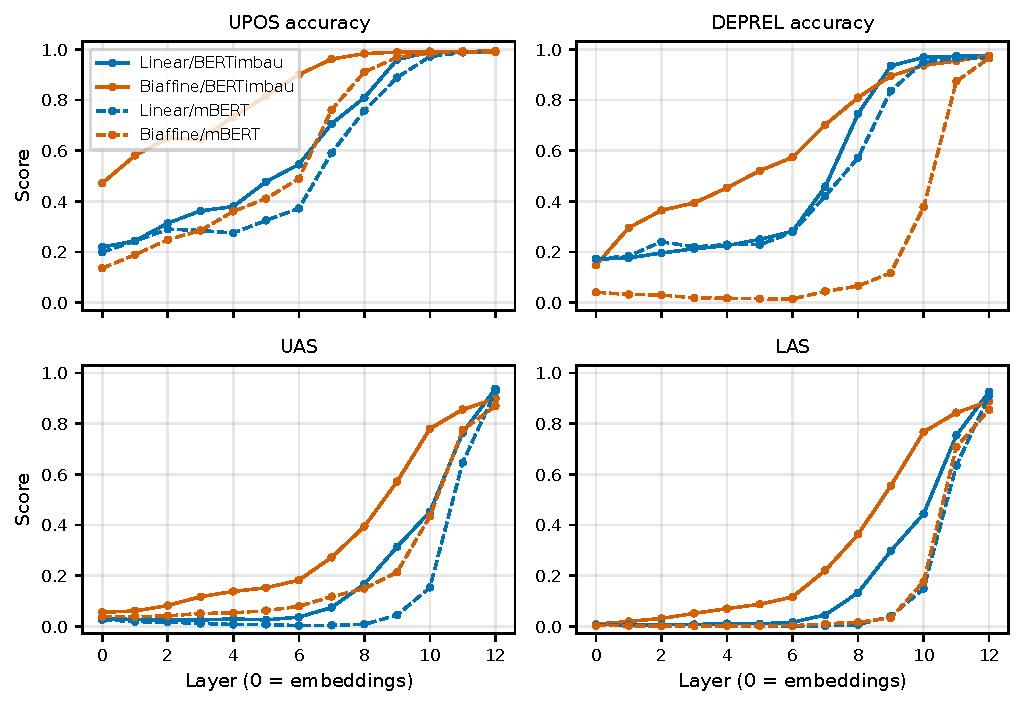
\includegraphics[width=0.95\textwidth]{imagens/layerwise_fig_per_layer.pdf}
\caption{Logit-lens read-out per layer for the four base models (95\% CI,
paired bootstrap). The pipeline ordering is universal; its depth is not.}
\label{fig:per-layer}
\end{figure*}

\begin{figure*}[t]
\centering
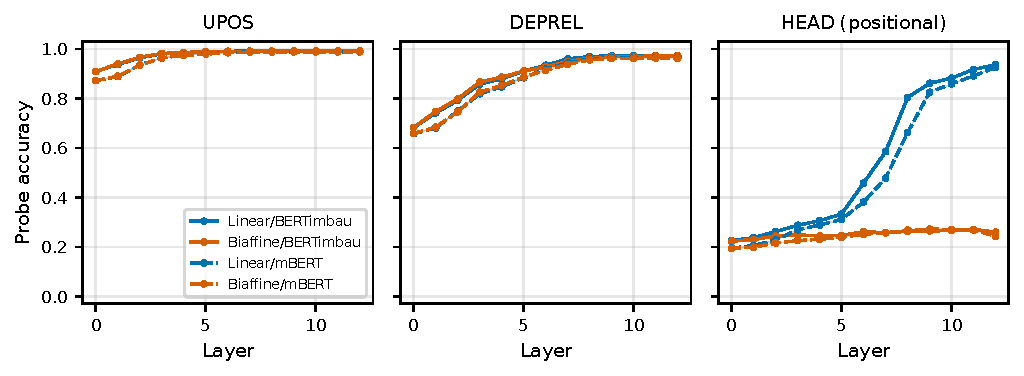
\includegraphics[width=0.95\textwidth]{imagens/layerwise_fig_probes.pdf}
\caption{Per-layer trained probes (5 seeds, $\pm\sigma$). UPOS and DEPREL
information is early and architecture-invariant; positional HEAD information
exists only in encoders fine-tuned by a linear (positional) decoder.}
\label{fig:probes}
\end{figure*}

\begin{figure}[t]
\centering
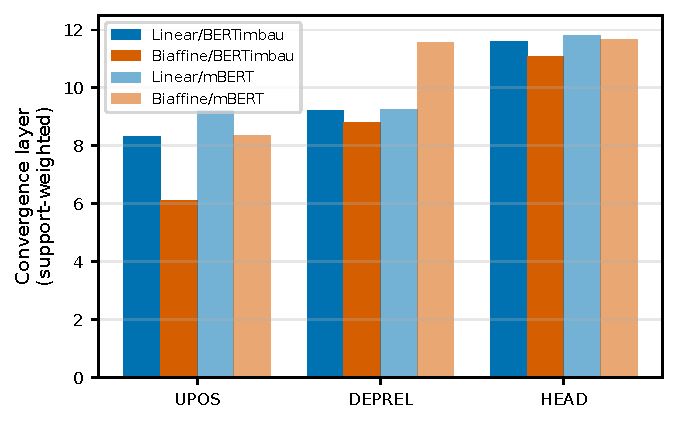
\includegraphics[width=0.95\columnwidth]{imagens/layerwise_fig_task_depth.pdf}
\caption{Support-weighted convergence layer per task and model.}
\label{fig:task-depth}
\end{figure}

\begin{figure}[t]
\centering
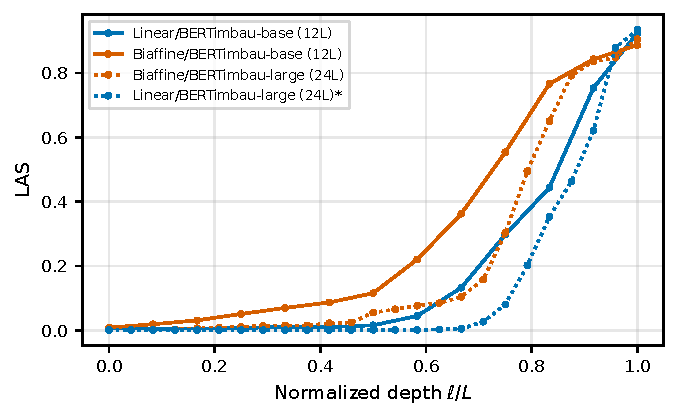
\includegraphics[width=0.95\columnwidth]{imagens/layerwise_fig_scale.pdf}
\caption{LAS vs.\ normalized depth $\ell/L$: 12- and 24-layer models overlap;
syntax resolves in the top quarter at both scales. (*) independent run.}
\label{fig:scale}
\end{figure}

\begin{figure}[t]
\centering
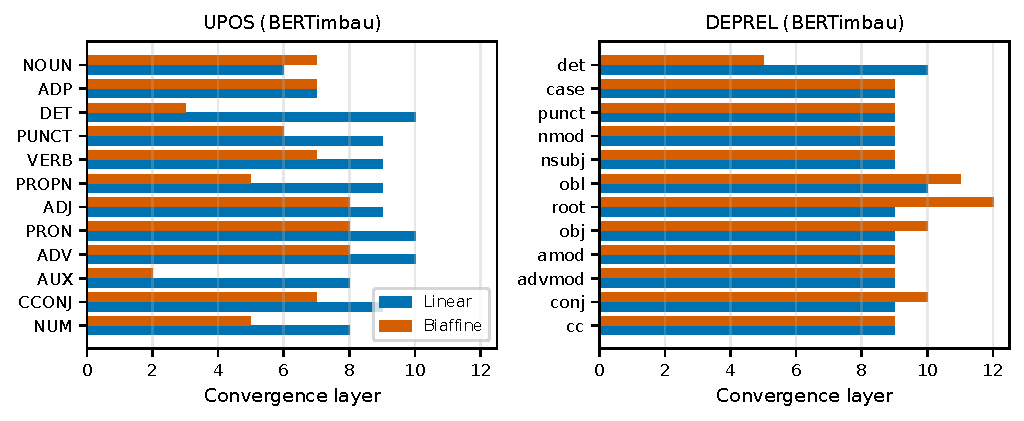
\includegraphics[width=0.95\columnwidth]{imagens/layerwise_fig_convergence.pdf}
\caption{Per-tag convergence layers (BERTimbau): closed-class ambiguous tags
resolve late; lexically cued tags resolve early.}
\label{fig:convergence}
\end{figure}

% ── TABELAS ────────────────────────────────────────────────────────────────────
% Todas geradas programaticamente — não editar à mão:
% Gerado por layerwise_comparison_aaai.py — não editar manualmente
% Requer: \usepackage{booktabs, multirow}

\begin{table}[t]
\centering
\caption{Layer-wise read-out (logit lens) on the Porttinari test set (1,683 sentences, 33,580 tokens). Heads are trained on layer~12; early exit reads all tasks from layer $L$.}
\label{tab:early-exit}
\begin{tabular}{llcccc}
\toprule
Model & $L$ & UPOS & DEPREL & UAS & LAS \\
\midrule
\multirow{5}{*}{Linear/BERTimbau} & 12 (full) & 99.22 & 97.33 & 93.74 & 92.49 \\
 & 11 & 99.06 & 97.26 & 76.34 & 75.33 \\
 & 10 & 98.92 & 96.81 & 45.18 & 44.34 \\
 & 9 & 95.96 & 93.47 & 31.34 & 29.73 \\
 & 8 & 80.90 & 74.58 & 16.58 & 13.23 \\
\midrule
\multirow{5}{*}{Biaffine/BERTimbau} & 12 (full) & 99.27 & 97.49 & 89.84 & 88.71 \\
 & 11 & 99.20 & 95.41 & 85.55 & 84.31 \\
 & 10 & 99.13 & 93.62 & 77.95 & 76.65 \\
 & 9 & 98.88 & 89.47 & 57.11 & 55.39 \\
 & 8 & 98.29 & 80.94 & 39.37 & 36.25 \\
\midrule
\multirow{5}{*}{Linear/mBERT} & 12 (full) & 98.88 & 96.63 & 92.70 & 91.04 \\
 & 11 & 98.78 & 96.48 & 64.57 & 63.42 \\
 & 10 & 97.09 & 95.02 & 15.27 & 14.82 \\
 & 9 & 88.86 & 83.66 & 4.41 & 3.93 \\
 & 8 & 75.75 & 57.19 & 0.73 & 0.56 \\
\midrule
\multirow{5}{*}{Biaffine/mBERT} & 12 (full) & 98.93 & 96.55 & 86.92 & 85.42 \\
 & 11 & 98.89 & 87.35 & 77.46 & 70.78 \\
 & 10 & 98.48 & 37.67 & 43.36 & 17.62 \\
 & 9 & 96.85 & 11.71 & 21.37 & 3.22 \\
 & 8 & 91.06 & 6.59 & 14.89 & 1.52 \\
\bottomrule
\end{tabular}
\end{table}

\begin{table}[t]
\centering
\caption{Final-layer contrasts with 95\% CI and two-sided $p$-values from a paired bootstrap over sentences (10,000 resamples; shared resample indices).}
\label{tab:significance}
\begin{tabular}{llcc}
\toprule
Contrast & Metric & $\Delta$ [95\% CI] & $p$ \\
\midrule
Biaffine $-$ Linear (BERTimbau) & UPOS accuracy & +0.04 [-0.03, +0.12] & 0.2482 \\
 & DEPREL accuracy & +0.16 [+0.01, +0.31] & 0.0382 \\
 & UAS & -3.91 [-4.50, -3.33] & $<$0.0001 \\
 & LAS & -3.78 [-4.38, -3.20] & $<$0.0001 \\
\midrule
Biaffine $-$ Linear (mBERT) & UPOS accuracy & +0.05 [-0.04, +0.15] & 0.2898 \\
 & DEPREL accuracy & -0.08 [-0.24, +0.08] & 0.3362 \\
 & UAS & -5.78 [-6.47, -5.10] & $<$0.0001 \\
 & LAS & -5.62 [-6.30, -4.94] & $<$0.0001 \\
\midrule
BERTimbau $-$ mBERT (Linear) & UPOS accuracy & +0.34 [+0.24, +0.44] & $<$0.0001 \\
 & DEPREL accuracy & +0.69 [+0.52, +0.87] & $<$0.0001 \\
 & UAS & +1.04 [+0.52, +1.57] & $<$0.0001 \\
 & LAS & +1.45 [+0.92, +1.98] & $<$0.0001 \\
\midrule
BERTimbau $-$ mBERT (Biaffine) & UPOS accuracy & +0.33 [+0.23, +0.43] & $<$0.0001 \\
 & DEPREL accuracy & +0.94 [+0.74, +1.14] & $<$0.0001 \\
 & UAS & +2.92 [+2.19, +3.62] & $<$0.0001 \\
 & LAS & +3.28 [+2.56, +4.00] & $<$0.0001 \\
\bottomrule
\end{tabular}
\end{table}

\begin{table}[t]
\centering
\caption{Block-skip ablation (UPOS / LAS): embeddings fed directly into a subset of encoder blocks. Depth is compositional: the last block alone, or iterated, fails across architectures and pretraining regimes.}
\label{tab:block-skip}
\begin{tabular}{lcccc}
\toprule
 & \multicolumn{2}{c}{BERTimbau} & \multicolumn{2}{c}{mBERT} \\
\cmidrule(lr){2-3}\cmidrule(lr){4-5}
Active blocks & Linear & Biaffine & Linear & Biaffine \\
\midrule
All blocks (normal) & 99.22 / 92.49 & 99.27 / 88.71 & 98.88 / 91.04 & 98.93 / 85.42 \\
Block 12 only & 53.76 / 1.71 & 51.49 / 2.26 & 44.87 / 1.50 & 36.50 / 2.13 \\
Block 12 $\times$12 & 13.20 / 0.50 & 8.06 / 0.39 & 7.13 / 0.29 & 6.59 / 2.63 \\
Blocks 11--12 & 51.44 / 2.30 & 44.53 / 1.48 & 41.65 / 2.14 & 37.99 / 1.20 \\
Blocks 9--12 & 65.28 / 4.68 & 63.00 / 4.06 & 47.11 / 3.41 & 44.96 / 2.68 \\
Blocks 7--12 & 71.38 / 9.30 & 68.43 / 7.22 & 60.01 / 6.76 & 63.75 / 4.01 \\
None (embeddings) & 21.92 / 0.74 & 47.10 / 0.80 & 19.89 / 0.60 & 13.58 / 0.20 \\
\bottomrule
\end{tabular}
\end{table}

\begin{table}[t]
\centering
\caption{Support-weighted mean convergence layer per task (first layer with acc $\geq 95\%$ of final).}
\label{tab:convergence}
\begin{tabular}{lccc}
\toprule
Model & UPOS & DEPREL & HEAD \\
\midrule
Linear/BERTimbau & 8.3 & 9.2 & 11.6 \\
Biaffine/BERTimbau & 6.1 & 8.8 & 11.1 \\
Linear/mBERT & 9.2 & 9.2 & 11.8 \\
Biaffine/mBERT & 8.4 & 11.6 & 11.7 \\
\bottomrule
\end{tabular}
\end{table}

\begin{table}[t]
\centering
\caption{Replication across independent training runs (ablation checkpoints trained without the UPOS head). Half-resolution depth = first layer with UAS $\geq 50\%$ of its final value.}
\label{tab:replication}
\begin{tabular}{lcccc}
\toprule
 & \multicolumn{2}{c}{LAS} & \multicolumn{2}{c}{Half-res.\ layer} \\
\cmidrule(lr){2-3}\cmidrule(lr){4-5}
Model & Main & Indep. & Main & Indep. \\
\midrule
Linear/BERTimbau & 92.49 & 92.23 & 11 & 11 \\
Biaffine/BERTimbau & 88.71 & 89.71 & 9 & 9 \\
Linear/mBERT & 91.04 & 90.81 & 11 & 11 \\
\bottomrule
\end{tabular}
\end{table}

\begin{table}[t]
\centering
\caption{Information vs.\ behavior: layer at which each read-out reaches 95\% of its final value. Per-layer trained probes (5 seeds, $\sigma \leq 0.003$) locate information much earlier than the deployed logit-lens read-out, and the biaffine encoder stores head attachment in a relational format invisible to single-token probes (final probe accuracy in parentheses).}
\label{tab:probes}
\begin{tabular}{llcc}
\toprule
Model & Task & Probe & Logit lens \\
\midrule
Linear/BERTimbau & UPOS & 2 (99.21) & 9 \\
 & DEPREL & 6 (97.35) & 9 \\
 & HEAD & 11 (93.68) & 12 \\
\midrule
Biaffine/BERTimbau & UPOS & 2 (99.26) & 7 \\
 & DEPREL & 6 (97.14) & 10 \\
 & HEAD & 3 (25.95) & 11 \\
\midrule
Linear/mBERT & UPOS & 3 (98.88) & 10 \\
 & DEPREL & 6 (96.62) & 10 \\
 & HEAD & 11 (92.64) & 12 \\
\midrule
Biaffine/mBERT & UPOS & 3 (98.93) & 9 \\
 & DEPREL & 7 (96.33) & 12 \\
 & HEAD & 5 (24.35) & 12 \\
\bottomrule
\end{tabular}
\end{table}

\begin{table}[t]
\centering
\caption{Head families retrained (3 seeds, mean; $\sigma \leq 0.003$) on the FROZEN 24-layer biaffine-fine-tuned encoder, at each task\textquotesingle s saturation layer. A freshly trained pairwise (biaffine) head recovers near-deployed attachment from intermediate layers; a freshly trained positional (linear) head cannot extract head positions from the same frozen representations at any depth. Deployed end-to-end MTL shown for reference.}
\label{tab:frozen}
\begin{tabular}{llcccc}
\toprule
Head & Layer & UPOS & DEPREL & UAS & LAS \\
\midrule
\multirow{4}{*}{Linear} & 10 (UPOS sat.) & 99.03 & 90.24 & 27.55 & 26.21 \\
 & 18 (DEPREL sat.) & 99.33 & 97.50 & 34.39 & 33.89 \\
 & 23 (HEAD sat.) & 99.34 & 97.68 & 30.42 & 30.03 \\
 & 24 (final) & 99.35 & 97.69 & 29.97 & 29.59 \\
\midrule
\multirow{4}{*}{Biaffine} & 10 (UPOS sat.) & 98.99 & 90.65 & 49.46 & 47.76 \\
 & 18 (DEPREL sat.) & 99.33 & 97.47 & 89.39 & 88.28 \\
 & 23 (HEAD sat.) & 99.33 & 97.60 & 91.10 & 89.99 \\
 & 24 (final) & 99.34 & 97.66 & 91.24 & 90.16 \\
\midrule
Deployed MTL & 24 (end-to-end) & 99.34 & 97.79 & 91.52 & 90.56 \\
\bottomrule
\end{tabular}
\end{table}


\bibliography{layerwise_aaai}

\end{document}
